% !TeX program = xelatex
\documentclass[UTF8,fontset=fandol,10pt,a4paper]{ctexart}
\usepackage[left=22mm,right=22mm,top=23mm,bottom=22mm,headheight=14pt]{geometry}
\usepackage{fontspec}
\setmainfont{TeX Gyre Heros}
\setsansfont{TeX Gyre Heros}
\setmonofont{Latin Modern Mono}
\renewcommand{\familydefault}{\sfdefault}
\usepackage[table]{xcolor}
\usepackage{graphicx,tikz}
\usetikzlibrary{arrows.meta,positioning,fit,backgrounds,calc}
\usepackage{booktabs,tabularx,array,enumitem,float,caption,fancyhdr,hyperref}
\definecolor{blue}{HTML}{2869A9}
\definecolor{ink}{HTML}{293340}
\definecolor{muted}{HTML}{647181}
\definecolor{line}{HTML}{C5D4E2}
\definecolor{pale}{HTML}{F0F5FA}
\definecolor{warm}{HTML}{FFF7E9}
\hypersetup{colorlinks=true,urlcolor=blue,linkcolor=blue,pdftitle={Redflag RHI 与 Vulkan 接入设计},pdfauthor={Redflag}}
\color{ink}
\setlength{\parindent}{0pt}
\setlength{\parskip}{6pt}
\linespread{1.16}
\setlist[itemize]{leftmargin=1.5em,itemsep=2pt,topsep=3pt}
\setlist[enumerate]{leftmargin=1.8em,itemsep=3pt,topsep=3pt}
\renewcommand{\arraystretch}{1.38}
\newcolumntype{Y}{>{\raggedright\arraybackslash}X}
\newcolumntype{L}[1]{>{\raggedright\arraybackslash}p{#1}}
\ctexset{section={format=\Large\bfseries\color{blue},beforeskip=16pt,afterskip=8pt},subsection={format=\large\bfseries\color{blue},beforeskip=11pt,afterskip=5pt}}
\captionsetup{font=small,labelfont=bf,textfont={color=muted},skip=7pt}
\pagestyle{fancy}\fancyhf{}
\fancyhead[L]{\small\color{muted}Redflag · RHI / Vulkan · 设计方案}
\fancyhead[R]{\small\color{muted}2026-11-21}
\fancyfoot[C]{\small\color{muted}\thepage}
\renewcommand{\headrulewidth}{0pt}
\newcommand{\note}[1]{{\small\color{muted}#1\par}}
\newcommand{\code}[1]{{\small\texttt{#1}}}
\newcommand{\ruleline}{\par\vspace{4pt}{\color{line}\hrule}\vspace{8pt}}
\newcommand{\source}[2]{{\small\href{#1}{[#2]}}}
\tikzset{
 module/.style={draw=line,fill=pale,rounded corners=2pt,align=center,inner sep=7pt,text width=3.8cm,minimum height=1.15cm,font=\small},
 smallbox/.style={module,text width=2.55cm,minimum height=.95cm,font=\footnotesize},
 wide/.style={module,text width=9.5cm},
 planned/.style={module,fill=warm,dashed},
 flow/.style={-{Stealth[length=2mm]},draw=muted,line width=.65pt},
 own/.style={flow,dashed},
 label/.style={font=\scriptsize,fill=white,inner sep=2pt,text=muted}}

% 本册的页幅、图注和代码排版。
\geometry{paperwidth=190mm,paperheight=252mm,left=21mm,right=21mm,
  top=22mm,bottom=21mm,headheight=21pt,headsep=4mm,footskip=10mm}
\usepackage{amsmath,listings,type1cm}
\definecolor{Ink}{HTML}{202E33}
\definecolor{Muted}{HTML}{4C6064}
\definecolor{Teal}{HTML}{12665F}
\definecolor{Rust}{HTML}{9E452B}
\definecolor{Rule}{HTML}{B3C6C1}
\definecolor{Soft}{HTML}{EAF3F0}
\definecolor{Paper}{HTML}{FFFFFF}
\setmainfont{TeX Gyre Pagella}
\renewcommand{\familydefault}{\rmdefault}
\linespread{1}
\setcounter{secnumdepth}{0}
\setlength{\emergencystretch}{2em}
\setlength{\parindent}{0pt}
\setlength{\parskip}{5.8pt}
\ctexset{section={format=\raggedright\sffamily\bfseries\fontsize{23}{30}\selectfont\color{Ink},
    beforeskip=0pt,afterskip=9pt},
  subsection={format=\raggedright\sffamily\bfseries\fontsize{13}{18}\selectfont\color{Teal},
    beforeskip=8pt,afterskip=2pt}}
\hypersetup{urlcolor=Teal,linkcolor=Teal,bookmarksnumbered=false,
  pdfsubject={Redflag 渲染接口、后端实现与验证}}
\fancyhf{}
\setlength{\headwidth}{\textwidth}
\fancyhead[L]{\sffamily\fontsize{9.5}{12}\selectfont\bfseries\color{Teal}Redflag\enspace{\mdseries\color{Muted}图形引擎}}
\fancyhead[R]{\sffamily\small\color{Muted}RHI / Vulkan}
\renewcommand{\headrule}{\hbox to\headwidth{\color{Rule}\leaders\hrule height .55pt\hfill}}
\fancyfoot[L]{\small\sffamily\color{Muted}\nouppercase{\leftmark}}
\renewcommand{\sectionmark}[1]{\markboth{#1}{}}
\fancyfoot[R]{\large\sffamily\bfseries\color{Teal}\thepage}
\renewcommand{\code}[1]{{\ttfamily\fontsize{10.4}{14}\selectfont #1}}
\newcommand{\readings}[1]{\par\noindent{\sffamily\fontsize{9.6}{14}\selectfont
  \color{Muted}参考\enspace #1\par}}
\newcommand{\refitem}[2]{\href{#1}{#2}}
\newcommand{\figpanel}[2]{\begin{figure}[H]\centering\input{figures/#1}\caption{#2}\end{figure}}
\DeclareCaptionFont{rhicapt}{\sffamily\fontsize{10}{14}\selectfont\color{Muted}}
\captionsetup{font=rhicapt,labelfont={bf,color=Teal},textfont=rhicapt,
  labelsep=quad,justification=raggedright,singlelinecheck=false,skip=4pt}
\setlength{\intextsep}{7pt plus 1pt minus 1pt}
\lstset{basicstyle=\ttfamily\fontsize{10.7}{15}\selectfont\color{Ink},
  backgroundcolor=\color{Soft},frame=l,rulecolor=\color{Teal},framerule=1.5pt,
  xleftmargin=5mm,xrightmargin=2mm,framexleftmargin=3mm,framesep=2pt,
  aboveskip=6pt,belowskip=6pt,columns=fullflexible,keepspaces=true,showstringspaces=false}
\newcommand{\bodytype}{\normalfont\fontsize{11.4}{17.8}\selectfont\color{Ink}}

\geometry{a4paper,left=22mm,right=22mm,top=20mm,bottom=19mm}
\setlength{\headwidth}{\textwidth}
\setlength{\parindent}{2\ccwd}
\setlength{\parskip}{6pt}
\ctexset{section={afterindent=true},subsection={afterindent=true}}
\fancyhead[R]{\sffamily\small\color{Muted}角色动画 / GAMES105}
\hypersetup{pdftitle={Redflag 角色动画},pdfsubject={骨骼、蒙皮与物理行走}}
\graphicspath{{../../../output/validation/character-animation/}}
\newcommand{\shot}[2]{\begin{figure}[H]\centering\includegraphics[width=.83\linewidth]{#1}\caption{#2}\end{figure}}
\newcommand{\clipref}[2]{\href{https://github.com/GAMES-105/GAMES-105/tree/442b13ad9c50544889236d6541358c9c752f8458/#1}{#2}}
\begin{document}
\bodytype
\section{场景里的骨骼动画}
在 Redflag Forge 的“文件 → 打开场景”中选择 \path{assets/scenes/Character-Walk.redflag}。角色会在地面中央循环走动。点击层级中的“角色”，属性面板的“骨骼动画”会显示当前动作。取消“循环播放”可以停住，拖动“进度（秒）”能观察膝盖抬到哪里。此时保存场景，再从同一个文件打开，角色会停在刚才的姿势。

\shot{scene.png}{正式 Vulkan 编辑器的场景面板，取自 RenderDoc 1.47 回放第 24 帧，640 × 410 像素。两只脚的位置和膝盖的弯曲来自课程提供的 \code{Walk.bvh}。}

要在自己的场景使用，先建一个空对象，在“添加组件”中选“骨骼动画”，再点“选择 BVH 动作”。示例文件在 \path{assets/animations/GAMES105/}。此组件以米读取骨架，人物按实体的平移、旋转和缩放摆放。它保留骨盆的上下运动，固定根关节在地面上的位置，适合从同一机位检查循环步态。

动作文件保存每个关节相对父关节的变化。\code{SkeletonAnimationComponent::Seek} 先在相邻动作帧间插值，再把各关节换算到角色坐标中。绘制时，一块细长的立方体连接两个相邻关节，19 根骨段都使用角色的拾取编号。这样，点中手或脚，属性面板都选中同一角色。在 Vulkan 光照视图里，骨段移动只需重画相机看到的表面。房间的烘焙仍可用，光线查询静态遮挡时只考虑房间里的静态模型。

场景文件分别保存动作路径、播放开关和秒数。动作路径相对于场景文件，另存时重新计算。复制场景后，两份角色可以共用读入的动作，各自暂停或继续。实现见 \href{run:../../Redflag/src/Redflag/Animation/SkeletonAnimation.cpp}{\code{SkeletonAnimation.cpp}}。在仓库根目录运行 \path{tests/run_lighting_preview_edits.cmd}，加上 \code{--skeleton} 选项，可以重做保存、重开与拾取验证。下面的六项操作使用独立示例，其中带皮肤的角色和由关节力驱动的平地行走都在该示例中体验。

\clearpage
\section{角色与骨架}
在仓库根目录打开 \path{Open-Character-Animation.cmd}。窗口左侧有六项操作。先选“正向运动学 FK”，拖动角度滑块。转动左肩时，肘和手腕一起移动，右手和双脚留在原处。浅蓝色线段画出两关节间的骨头，橙色方块标出关节的位置。

\shot{fk.png}{Redflag 在 RTX 5070 Ti Laptop GPU 上绘制的独立 Vulkan 动画示例。画面中的左肩转过 $-32^\circ$。数字键 1 至 6 也可以切换左侧的动作。以下的视口图均取自同一程序。}

骨架里共有 20 个关节。手腕只记录自己离肘有多远，以及相对肘转了多少。设肘在模型中的位置为 $p$，朝向为 $R$，从肘指向手腕的局部位移为 $d$。先把 $d$ 转到肘现在的朝向，再接到肘上，得到手腕位置 $p+Rd$。例如 $d=(0.24,0,0)$ 米时，肘绕 $Z$ 轴转 $90^\circ$，手腕便在肘上方 0.24 米。这种从父关节逐级求子关节位置的方法叫正向运动学（FK）。

\codewhere{源码}{Redflag/src/Redflag/Animation/Skeleton.cpp}{ToModelSpace}
\begin{lstlisting}[style=besidetext]
// (*@\rhicomment{父关节排在前面，计算手腕时已经知道肘在哪里。}@*)
model[i].Position = model[parent].Position
                  + model[parent].Rotation * local[i].Position;
model[i].Rotation = glm::normalize(model[parent].Rotation
                                  * local[i].Rotation);
\end{lstlisting}

从源码首次运行时，在仓库根目录用 PowerShell 准备物理库，再用 Visual Studio 生成 Debug/x64 的 RedflagForge。演示首次启动会编译示例，需要同一套 MSVC 和 Vulkan SDK。
\begin{lstlisting}[style=besidetext]
.\scripts\BuildPhysX.ps1 -Configuration Debug
\end{lstlisting}
改完引擎之后重新生成项目，再运行 \path{tests/run_character_animation.cmd} 验证。

\clearpage
\section{手腕的位置}
选择“逆向运动学 IK”，移动金色方块。手腕要到达给定位置，上臂和前臂仍须保持原来的长度。仅给手腕一个目标，肘可以从不同方向弯过去，所以接口还接收一个参考点 \code{pole}，例如放在肩膀的左下方。

\begin{figure}[H]\centering
\begin{minipage}[c]{.56\linewidth}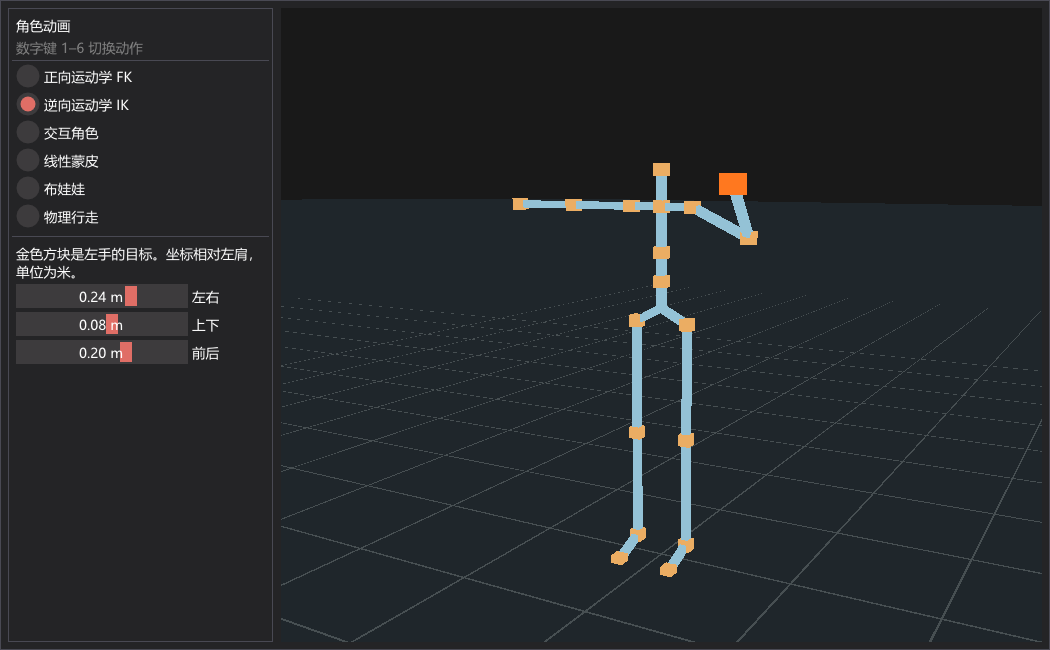
\includegraphics[width=\linewidth]{ik.png}\end{minipage}\hfill
\begin{minipage}[c]{.40\linewidth}\centering
\begin{tikzpicture}[scale=.89, line cap=round,font=\small]
\coordinate (A) at (0,0); \coordinate (B) at (2,2.24); \coordinate (C) at (4,0);
\draw[Teal,line width=1.3pt] (A)--node[left]{$a$}(B)--node[right]{$b$}(C);
\draw[Muted] (A)--(C);\draw[Rust,dashed] (B)--node[right]{$h$}(2,0);
\draw[Muted] (1.84,0)--(1.84,.16)--(2,.16);
\draw[Muted,|<->|] (0,-.48)--node[below]{$x$}(2,-.48);
\draw[Muted,|<->|] (0,-.98)--node[below]{$d$}(4,-.98);
\fill[Teal] (A) circle (2pt) node[left]{肩};
\fill[Teal] (B) circle (2pt) node[above]{肘};
\fill[Rust] (C) circle (2pt) node[right]{目标};
\end{tikzpicture}\end{minipage}
\caption{左图的滑块设定目标相对肩膀的距离。右图是本文按两条骨长画的示意，虚线是肘到肩腕连线的垂直距离。目标再远过臂长，上下臂就会伸直。}
\end{figure}

把肩、肘和目标画成一个三角形。上臂长 $a$，前臂长 $b$，肩到目标的距离为 $d$。沿肩到目标的直线，肘的投影离肩 $x$，垂直离开这条线的距离为 $h$。分别对两条手臂写勾股定理，得到 $a^2=x^2+h^2$ 和 $b^2=(d-x)^2+h^2$。两式相减，求出
\[
       x=\frac{a^2+d^2-b^2}{2d},\qquad h=\sqrt{a^2-x^2}.
\]
例如两段各长 $0.3$ 米，目标在肩前方 $0.4$ 米。代入可得 $x=0.2$ 米，$h\approx0.224$ 米。沿目标方向走 $0.2$ 米，再朝参考点所在的一侧走 $0.224$ 米，这就是肘的位置。$d$ 大于 $a+b$ 时，以臂长为最远距离；$d$ 小于 $|a-b|$ 时，两段折叠到能达到的最近处。

\codewhere{调用示例}{examples/CharacterAnimation/CharacterDemo.cpp}{Demo::Draw}
\begin{lstlisting}[style=besidetext]
// (*@\rhicomment{target 和 pole 均以角色模型为坐标系。结果写回局部姿势。}@*)
rig.SolveTwoBone(local, rig.Find("lWrist"), target, pole);
Pose model = rig.ToModelSpace(local);
\end{lstlisting}

测试选择了一处手臂够得到的目标。求解前，手腕离目标 0.643292 米；求解后相差 $1.19\times10^{-7}$ 米。另一次把目标放在三米外，测试核对伸直后的肩腕距离是否等于两段骨长之和。

\clearpage
\section{站立、起步与转向}
选择“交互角色”，按 W、A、S、D 移动。根关节在骨盆附近。它的水平位置决定角色走到哪里，姿势里的其他关节决定这一步怎样迈出去。示例采用课程发布的两段 BVH 动作。行走片段有 100 帧，每隔 0.01 秒记录一次；站立片段有 200 帧，每隔约 0.016667 秒记录一次。两段都有骨盆和四肢的动作。

\shot{move.png}{使用正常交互入口选择“交互角色”后，在窗口按住 W 的实拍。身体网格由项目根据骨长生成，动作数据取自课程的公开文件。}

\code{AnimationClip::LoadBVH} 先读文件开头的关节名称、父子关系和初始距离，再按文件列出的顺序读取平移或转角。BVH 存的角度用度表示，创建四元数前转换为弧度。若当前时间落在第 3 帧和第 4 帧正中，位置取两者中点。旋转则沿两个朝向之间的较短圆弧走一半，手臂弯到中间时骨头长度不变。

角色每秒沿 $X$ 走 0.6 米、沿 $Z$ 走 0.8 米，一秒内实际走过 $\sqrt{0.6^2+0.8^2}=1$ 米。两秒后水平位置为 $(1.2,1.6)$ 米。程序把输入速度乘帧间隔，加到当前位置。同时用行走片段中骨盆的首尾水平位移除以记录时长，估计拍摄这段动作时的速度。输入变快时，也让动作更快跨过同一段步态。循环接回第一帧时，用已经走到的水平位置替换记录里的起点，骨盆上下的起伏则原样保留。

\codewhere{源码}{Redflag/src/Redflag/Animation/CharacterController.cpp}{Update，摘录}
\begin{lstlisting}[style=besidetext]
m_Position += velocity * seconds;     // (*@\rhicomment{世界坐标中的水平位移，米。}@*)
m_WalkTime += seconds * speed / m_ClipSpeed;
Pose walk = m_Walk.Sample(m_WalkTime);
\end{lstlisting}

松开键盘时，两段动作在每一帧重新混合。代码选用的 0.12 秒是指数变化的时间常数，经过这段时间后，身体大约完成两种姿势之间 63\% 的过渡。转向也沿较短的角度改变朝向。角色在地面上的水平速度由玩家直接给定，这一模式适合练习动作切换；碰撞和受力行走见后两页。

\clearpage
\section{骨头带动网格}
选择“线性蒙皮”，拖动步态滑块，观察小腿和前臂。网格保存的是初始姿势下的顶点。一个顶点最多记四个关节的编号和各自所占的权重，权重之和为 1。靠近关节时，相邻骨头都能影响同一个点。

\shot{skin.png}{步态滑块停在 0.27 秒的 Vulkan 画面。蓝色和金色区分两组网格区域。颜色中的明暗是示例贴图，用来观察轮廓。}

初始姿势下，某个顶点在 $p$，第 $j$ 块骨头从 $b_j$ 转到 $R_j$、移至 $t_j$。这里 $b_j$ 是该关节在初始模型中的位置，初始旋转是单位旋转。先用 $p-b_j$ 表示顶点在骨头旁的位置，再跟着骨头转，最后加上新的关节位置。各关节给出的结果按权重 $w_j$ 混合：
\[
             p'=\sum_j w_j\,[\,R_j(p-b_j)+t_j\,].
\]
测试中一个顶点有 25\% 随第一块骨头，75\% 随第二块。第一块不动，第二块沿 $X$ 移动 0.8 米，顶点便移动 $0.75\times0.8=0.6$ 米。表面法线只跟着旋转。混合后的向量长度会变，所以还要把非零法线重新归一化。

\codewhere{示例}{examples/CharacterAnimation/CharacterDemo.cpp}{Demo::Draw，省去材质和视图代码}
\begin{lstlisting}[style=besidetext]
// (*@\rhicomment{CPU 计算这次姿势的顶点，原网格与三角形编号仍可用于下一帧。}@*)
surface = m_Draw.CreateMesh(m_Skin.Deform(model), m_Skin.GetIndices());
// (*@\rhicomment{当前帧的 Vulkan 绘制保留 surface，显卡用完后才释放它。}@*)
m_Draw.DrawIndexed(surface, m_Colors, vp, glm::mat4(1), glm::vec4(1), 2);
\end{lstlisting}

每次变形都会上传顶点和索引。这使示例能直接使用已有 RHI 的网格接口，大量角色每帧如此上传会增加工作量。正式测试用 96×64 的图像绘制带两个关节权重的三角形，移动前在像素 $(48,32)$ 拾取到实体 39，移动后原处读到背景，$(77,32)$ 读到实体 39。

\clearpage
\section{肢体落地与物理行走}
切到“布娃娃”，髋、膝和踝在重力作用下落到地面。这个下半身由七个可移动的盒子组成，每个盒子都有自己的实体编号。髋、膝、踝处的六个关节把相邻盒子的连接点保持在一起，同时允许肢体绕左右方向的轴弯曲。用两组局部坐标指定同一个连接点，PhysX 就知道小腿的上端要接在哪一条大腿的下端。

\shot{walk.png}{“物理行走”的同机实拍。左侧速度是控制器想达到的速度。地面摩擦、关节驱动和骨盆辅助力共同决定实际走了多远。}

选择“物理行走”后，左右腿的动作相差半个周期。一条腿向前摆时，同侧膝盖弯曲，脚得到抬起的空间。每次模拟前，\code{DriveWalk} 给关节一个目标角。当前角度与目标的差越大，驱动越用力；角速度越大，阻尼越强。可用一根被扭转的弹簧理解这个过程。在一根固定的转轴上，若目标角速度为零，近似力矩为
\[
             \tau=k_p(\theta_{\rm target}-\theta)-k_d\dot\theta .
\]
代码给髋、膝和踝传入刚度 200（牛顿米/弧度）、阻尼 18（牛顿米秒/弧度）和力矩上限 160 牛顿米。这组数按示例肢体的米制尺寸试调；刚度越大越想贴近目标，阻尼越大越能抑制转动。实际力矩由 PhysX 的 D6 关节解算。世界按 $1/60$ 秒向前模拟，取出各盒子的新位置后再绘制。

关节照着角度走，骨盆仍可能倾倒。示例从脚附近向下查询静态地面。至少一只脚附近有地面时，角度弹簧扶正骨盆，骨盆低于站立高度时施加向上的力，并按前进速度之差给水平推力。腾空时关闭这些辅助。课程作业也把根部受力和仅靠脚部关节平衡分开练习。本例实现有辅助的平地行走，斜坡、动态地面、只靠脚底推地保持平衡还有待验证。

\clearpage
\section{接口与验证}
运动学和物理各自保存一份能被绘制的姿势。前者用 \code{Pose} 的每个元素保存关节的平移和旋转，数组编号与骨架一致。后者使用 \code{PhysicsWorld::GetPose} 按稳定的实体编号取盒子的位置和朝向。表中每一行都能在演示或回归测试中找到调用点。

{\noindent\small\begin{tabularx}{\linewidth}{@{}p{55mm}X@{}}\toprule
接口 & 传入的数据与结果\\\midrule
\code{AnimationClip::Sample} & 秒数。返回局部关节姿势，可按 BVH 的时长循环。动作片段在控制器整个使用期内保留。\\
\code{Skeleton::ToModelSpace} & 局部姿势。结果按关节顺序给出模型坐标和朝向，蒙皮和骨架显示均可读取。\\
\code{Skeleton::SolveTwoBone} & 可写的局部姿势、末端编号、目标和参考点。末端上方须有两个关节，修改的是这两个关节的局部旋转。\\
\code{CharacterController::Update} & 本帧时长和 $XZ$ 平面上的速度。返回已混合的局部姿势，根关节含玩家指定的水平位移。\\
\code{SkinnedMesh::Deform} & 该骨架的模型空间姿势。返回 CPU 顶点数组，保留顶点 UV 和原有三角形顺序。\\
\code{Ragdoll::DriveWalk} & 固定时长与沿 $+Z$ 的目标速度。调用方再运行物理步，才得到新的刚体位置。\\
\code{Ragdoll::Relax} & 关闭肢体和骨盆的驱动，仍保留关节连接与重力。销毁角色时先释放关节，再移除各肢段。\\\bottomrule
\end{tabularx}\par}

物理测试把目标速度设为 0.8 米/秒，在平地上持续 6 秒，共模拟 360 步。角色实际前进 2.858 米，平均约 0.476 米/秒。跳过起步的半秒后，骨盆最低 0.860 米；左、右脚各有四次高出对侧脚至少 2.5 厘米。分别按脚盒的旋转计算最低点，330 个测量时刻中，左脚有 243 次距地面小于 5 毫米，右脚有 244 次。输入改为零后再过两秒，骨盆还前进了 0.286 米。另一项测试关闭全部驱动后自由下落，骨盆高度在三秒内从 1.91 米变为 0.504 米。

运行 \path{tests/run_character_animation.cmd} 可以重测。设置、设备、截图与实际读数在 \path{output/validation/character-animation/}，测试断言在 \path{tests/CharacterAnimationTests.cpp}。运动学的两米来自输入速度积分，物理模式的距离来自模拟后真实的骨盆位置。

\readings{\href{https://games-105.github.io/}{GAMES105 课程}第 3、4、8、9、10 讲。课程作业按 \clipref{lab1}{lab1 骨架}、\clipref{lab2}{lab2 动作与交互}、\clipref{labS}{labS 蒙皮}和\clipref{lab3}{lab3 物理角色}阅读。公开仓库将物理行走放在 \path{lab3/task2_physics_walker.py}。动作文件原样保留于 \path{assets/animations/GAMES105}。关节角度、约束轴与驱动参见 \href{https://nvidia-omniverse.github.io/PhysX/physx/5.6.1/docs/Joints.html}{NVIDIA PhysX 5.6.1 文档，Joints 与 D6 Joint}。}
\end{document}
